% results.tex
\documentclass[main.tex]{subfiles}
\begin{document}
\chapter{Results} \label{ch:res}

This chapter presents all the results stemming from the experimental procedures described in Chapter \ref{ch:exp}. Additionally, details are provided regarding proper data processing, and the calculations that lead to the definition of the desired failure surface. 

\section{Tensile Tests} \label{sec:tensr}
Performing tensile tests showed that the values of $X_t$ and $Y_t$ were significantly different, in accordance to the literature review presented in Section \ref{ssec:mechPropFFF}. An initial number of 20 samples per orientation was produced, however, multiple specimens failed outside the gage section of the coupon and thus, data originating from these coupons was considered invalid and promptly discarded. The valid results are summarized in Table \ref{tab:tensrtab}. Note that $X_t$ was on average 9.16 MPa higher than $Y_t$, a difference of 22.7\%.
\begin{table} [h]
	\centering
	\caption{Summary of Tensile tests}
\begin{tabular}{ c| c c } 
	\toprule
	\textbf{Information} & $X_t$ & $Y_t$\\
	\midrule
	Average [MPa] & 40.29 & 31.13\\
	Standard Deviation & 0.75 & 0.58\\
	Number of samples & 19 & 12\\
	Lowest measurement [MPa] &39.37  & 29.68\\
	Highest measurement [MPa] &40.90 & 32.08\\
	\bottomrule
\end{tabular}
\label{tab:tensrtab}
\end{table}

The behavior of both sets of samples was completely different. Coupons used to measure $X_t$ clearly showed whitening of the gage section, indicating plastic deformation. Specimens used for $Y_t$ on the other hand generally failed between beads and rarely showed any change in color. Figure~\ref{fig:tensComp} clearly shows the difference in mechanical behavior. Note how the $X_t$ specimen shows a ductile failure, as opposed to brittle breakage for the $Y_t$ sample.
\pagebreak

\begin{figure}[h]
	\center
	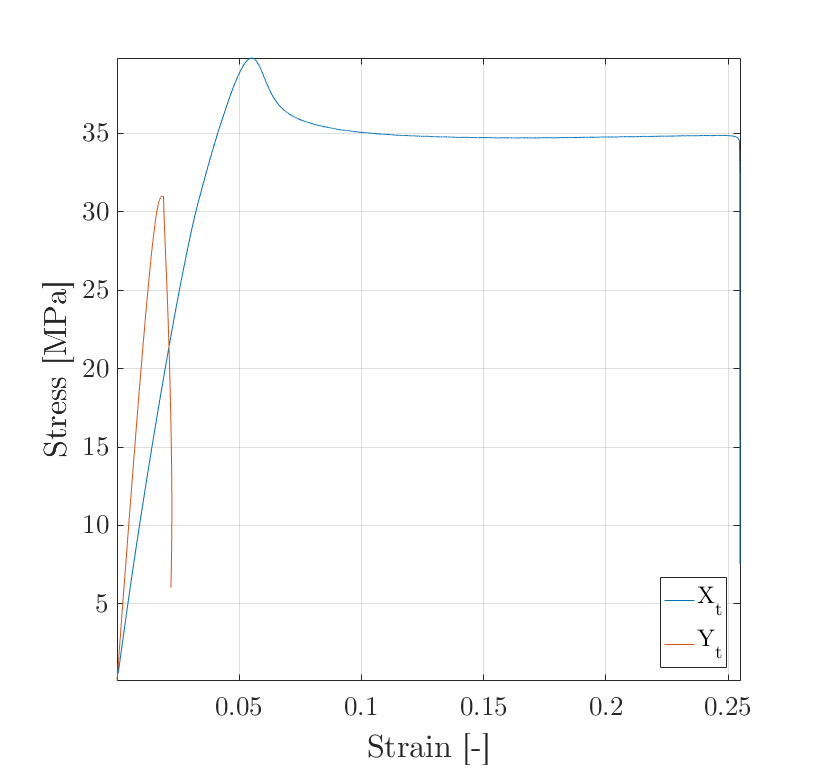
\includegraphics[height=9cm, keepaspectratio]{tenscomp}
	\caption{Comparison of tensile results} \label{fig:tensComp}
\end{figure}

Anderson-Darling tests (ADT) were performed on the results to validate if the data follows a normalized distribution. In the case of $X_t$, the ADT yields a p-value of 0.023. Thus, on a 95\% confidence interval, a normalized distribution can be discarded. This can be seen graphically in the goodness of fit plot, where data points fail to align with the slope that corresponds to a theoretical Gaussian distribution. By contrast, performing the ADT on the $Y_t$ samples fails to reject a normalized distribution using the same confidence interval, offering a p-value of 0.109. A case could be made for a false negative for $X_t$ and a false positive for $Y_t$, given the relatively small sample size for each data set. The results from ADT can be seen in Figure \ref{fig:adttens}.

\begin{figure}[!htbp]
	\center
	\subfloat[$X_t$ \label{fig:adtxt}]{%
		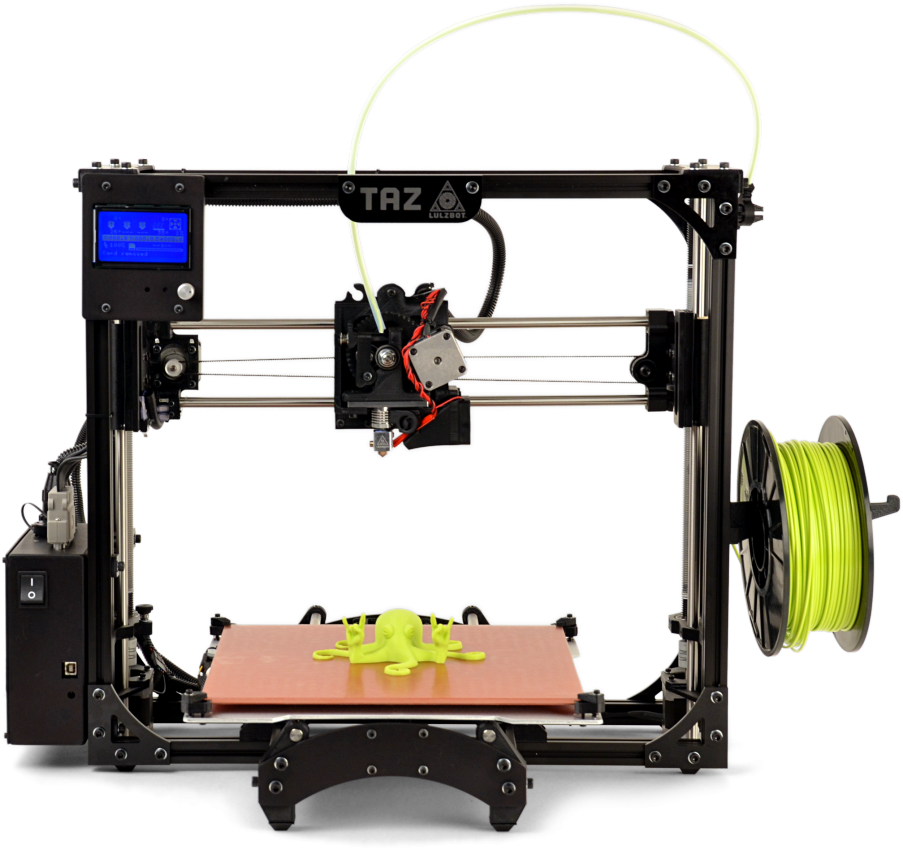
\includegraphics[height=4cm, keepaspectratio]{TAZ_5}
	}
	\hfill
	\subfloat[$Y_t$\label{fig:adtyt}]{%
		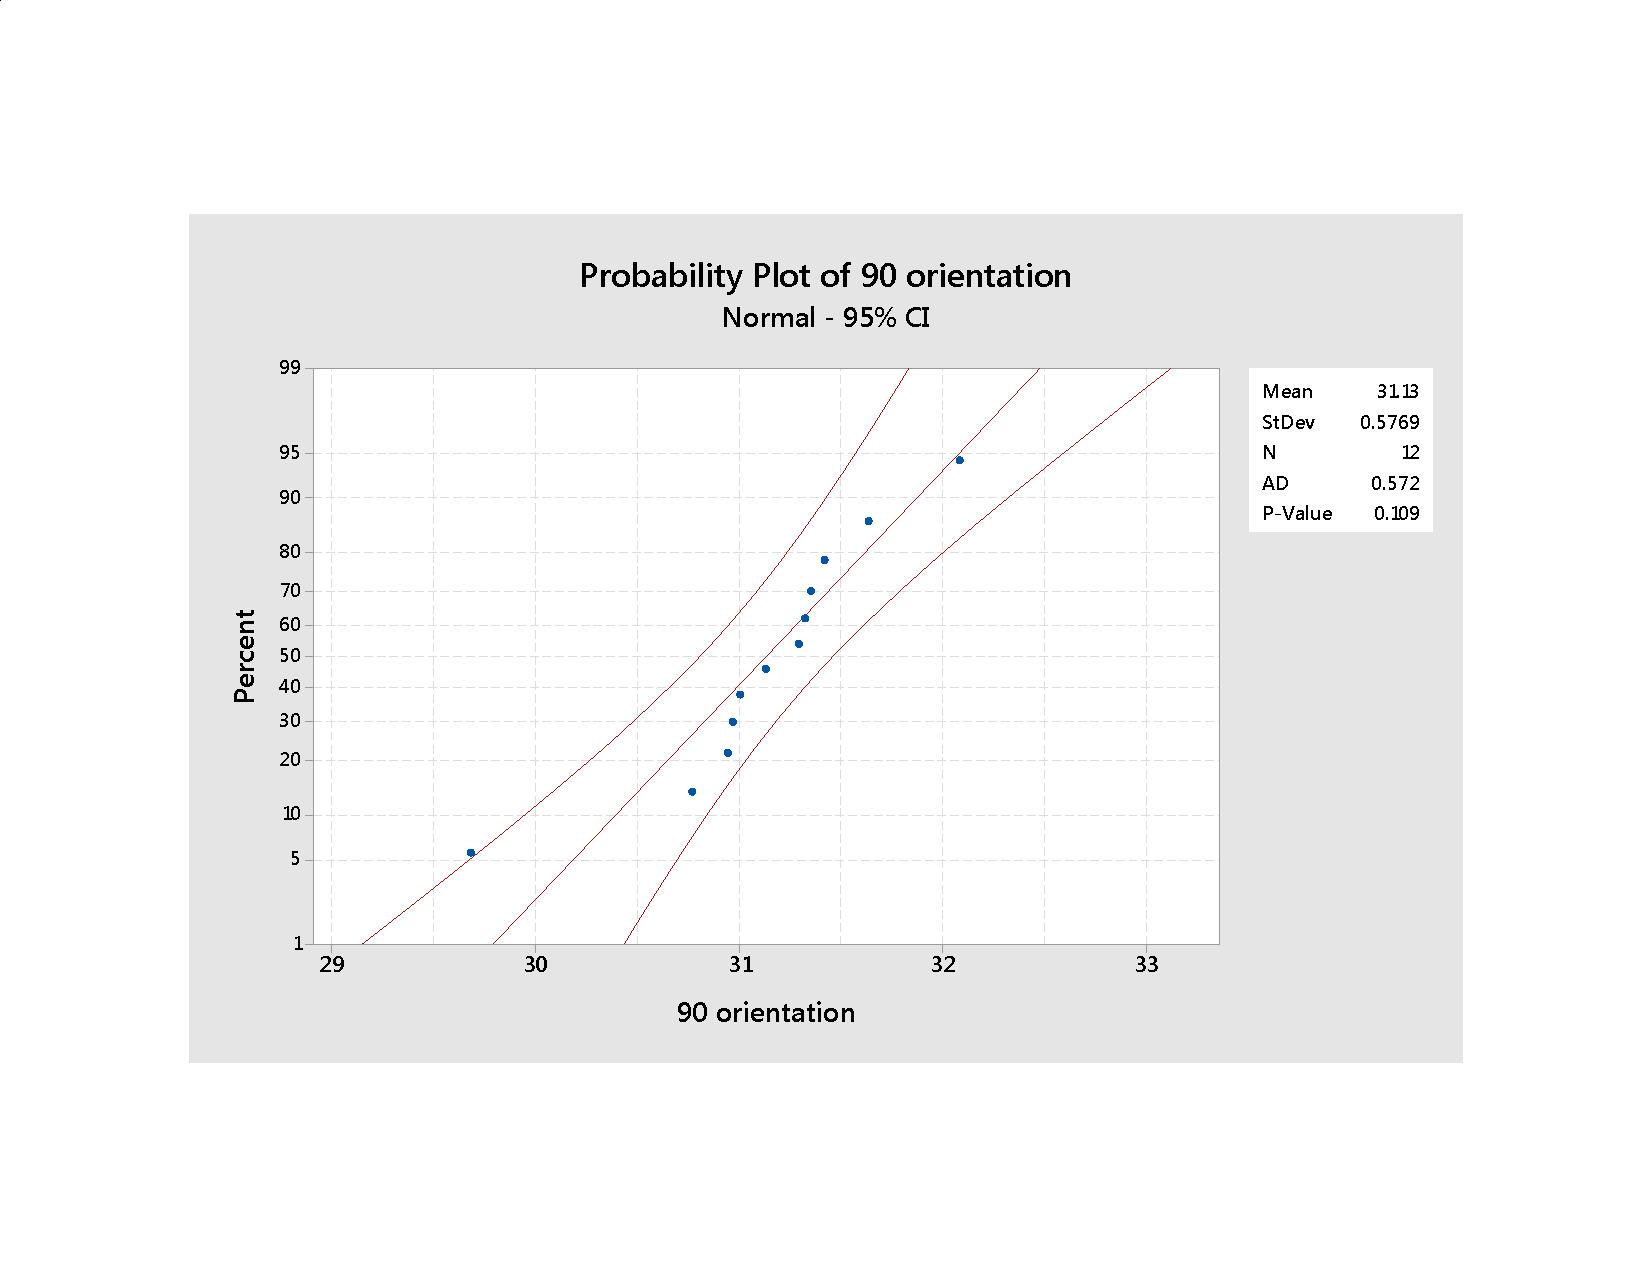
\includegraphics[height=4cm, keepaspectratio]{ADTyt.pdf}
	}
	\caption{ADT results} \label{fig:adttens}
\end{figure}
      
\section{Compression Tests} \label{sec:compr}
For the compression tests, a total of 25 samples were produced for each orientation. However, a number of coupons were discarded due to manufacturing defects. Table \ref{tab:comprtab} summarizes the test results.  

\begin{table} [h]
	\centering
	\caption{Summary of Compression tests}
	\begin{tabular}{ c| c c } 
		\toprule
		\textbf{Information} & $X_c$ & $Y_c$\\
		\midrule
		Average [MPa] &  & 57.96\\
		Standard Deviation &  & 1.81\\
		Number of samples &  & 22\\
		Lowest measurement [MPa] & &54.93 \\
		Highest measurement [MPa] & &61.39 \\
		\bottomrule
	\end{tabular}
\label{tab:comprtab}
\end{table}

The $Y_c$ samples displayed ductile behavior through testing. A clear maximum stress can be observed at the yield point in a stress-strain graph. The tubular samples showed localized whitening and deformation along portions of the tubular geometry.

Performing an ADT on the $Y_c$ samples reveals a p-value of 0.072, thus a normalized distribution cannot be discarded on a 95\% confidence interval. 

\section{Torsion Tests} \label{sec:torsr}
\subsection{45$^\circ$ orientation} \label{ssec:45r}
A total of 30 samples were produced with a 45$^\circ$ bead orientation, divided evenly for tests in positive and negative shear. As was the case for tensile and compressive tests, a number of specimens had to be discarded due to undesired behavior during testing. A common problem was delamination of the grips, thus requiring the data to be discarded. 

Results showed significant difference in behavior depending on the direction of the applied torque. The $S_{45p}$ samples showed a completely brittle behavior, fracturing between beads, as opposed to ductile failure in the center of the specimen for the $S_{45n}$ coupons. This resulted in an average difference of 6.3 MPa between both sets of data. Results are summarized in Table \ref{tab:tors45r}.

\begin{table} [h]
	\centering
	\caption{Summary of 45$^\circ$ torsion tests}
\begin{tabular}{ c| c c } 
	\toprule
	\textbf{Information} & $S_{45p}$ & $S_{45n}$\\
	\midrule
	Average [MPa] & 20.80 & 27.13\\
	Standard Deviation & 2.50 & 0.50\\
	Number of samples & 9 & 9\\
	Lowest measurement [MPa] &17.21  & 26.59\\
	Highest measurement [MPa] &24.61 & 28.17\\
	\bottomrule
\end{tabular}
\label{tab:tors45r}
\end{table}
  
\subsection{0$^\circ$ orientation} \label{ssec:0r}
\subsection{90$^\circ$ orientation} \label{ssec:90r}
\section{Combined Loading Tests} \label{sec:clr}
\section{Development of the Failure Surface} \label{sec:fsc}

The failure surface calculations were performed using MATLAB\textregistered~code based on previous work by Obst \emph{et al.} \cite{Obst2018}. This code can be found in Appendix \ref{ch:fsurfcode} for reference.

Calculations were based on the average values obtained from the mechanical tests to incorporate a probabilistic approach to the failure surface as developed by Zaitsev, Pashkov and Strelyaev \cite{Zaitsev1975}. This implies that the condition $f=1$ in Equation \ref{eq:GKCfinal} is equivalent to a probability of part failure of 50\%, since mean values of mechanical strength were used to calculate the tensorial components of the failure envelope.  

% Nomenclature introduced in this chapter:
\nomenclature[A]{ADT}{Anderson-Darling Test}% 

% Symbols introduced in this chapter:
%\nomenclature[S]{$\epsilon$}{Engineering Strain \nomunit{$-$}}%
\end{document}